\newpage		
\section*{Домашнее задание 2}
	\subsection*{Задача 1}
	\noindent
	\textbf{Условие}\\
	Найдите без помощи компьютера коэффициент при $q^{24640}$ в $q$-биноминальном коэффициенте $\left[\begin{array}{c}314 \\ 159\end{array}\right]_{q}$ \\
	\textbf{Решение}\\
	$q$-биноминальный коэффициент $\left[\begin{array}{c}m+n \\ m\end{array}\right]_{m+n}$ равен количеству диаграмм Юнга вписанных в прямоугольник $m\times n$\\
	Заметим, что производящая функция имеет вид $\left[\begin{array}{c}m+n \\ m\end{array}\right] = \sum\limits^{mn}_{k=0} = a_kq^k$.\\
	Заметим также что 
	\begin{gather*}
		\left[\begin{array}{c}314 \\ 159\end{array}\right]_{q} =
		\left[\begin{array}{c}159+155 \\ 159\end{array}\right]_{q}
	\end{gather*}
	То есть это диаграммы юнга вписанные в прямоугольник $159\times155$, его площадь $159 \cdot 155 = 24645$, следовательно коэффициент перед $q^{24640}$ равен количеству диаграмм Юнга из $24640$ или $24645-24640 = 5$ блоков. Диаграмм из $5$ блоков ровно $7$, а следовательно и коэффициент перед $q^{24640}$ -- $7$.\\
	\\
	\textbf{Ответ}: $7$\\
	
	
	\subsection*{Задача 2}
	\noindent
	\textbf{Условие}
	\begin{enumerate}
	\item[(a)] Докажите равенство
		\begin{gather*}
			(1+t)(1+t^2)(1+t^3)\ldots = \frac{1}{(1-t)(1-t^3)(1-t^5)\ldots}
		\end{gather*}
	\item[(б)] Докажите, что для каждого целого $n>0$ следующие два числа равны:
		\begin{enumerate}
		\item[$\bullet$] количество наборов целых чисел $(x_1, \ldots, x_k)$ (со всевозможными $k$), в которых\\
		$0 < x_1 < x_2 < \ldots < x_k$ и $x_1 + \ldots + x_k = n$
		\item[$\bullet$] количество наборов нечетных чисел $(y_1,\ldots,y_k)$ (со всевозможными $k$), в которых\\
		$0 \leqslant y_1 \leqslant y_2 \leqslant \ldots \leqslant y_k$ и $y_1 + \ldots + y_k = n$
		\end{enumerate}
	\end{enumerate}
	\textbf{Решение}\\
	\begin{enumerate}
	\item[(a)] 
		\begin{gather*}
			(1+t)(1+t^2)(1+t^3)\ldots = 
			\frac{(1-t^2)(1-t^4)(1-t^6)\ldots}{(1-t)(1-t^2)(1-t^3)\ldots} =\\
			\frac{1}{1-t} \cdot \frac{1-t^2}{1-t^2} \cdot \frac{1}{1-t^3} \cdot \frac{1-t^4}{1-t^4} \cdot \ldots = 
			\frac{1}{(1-t)(1-t^3)(1-t^5)\ldots}
		\end{gather*}
	\item[(б)]
		Обозначим за $A_0$ количество разбиений первого типа (на различные целые), а за $A_1$ второго типа (на нечетные числа).
		Тогда посчитаем производящие функции $A_0$ и $A_1$:
		\begin{gather*}
			A_0(t) = \sum A_0(n) t^n = 
			(1+t)(1+t^2)(1+t^3)\ldots\\
			A_1(t) = \sum A_1(n) t^n = 
			(1+t+t^2+\ldots)(1+t^3+t^6+\ldots)\ldots = 
			\frac{1}{1-t} \cdot \frac{1}{1-t^3} \cdot \ldots = 
			\frac{1}{(1-t)(1-t^3)(1-t^5)\ldots}
		\end{gather*}
		Остается заметить, что
		\begin{gather*}
			A_0(t) = (1+t)(1+t^2)(1+t^3)\ldots = \frac{1}{(1-t)(1-t^3)(1-t^5)\ldots} = A_1(t)
		\end{gather*}
	\end{enumerate}
	
	
	
	\newpage
	\subsection*{Задача 3}
	\noindent
	\textbf{Условие}\\
	Изобразите дерево на десяти вершинах, пронумерованных числами от $0$ до $9$, кодом Прюфера которого являются восемь цифр Вашего дня рождения, записанного в формате DD-MM-YYYY.\\
	\\
	\textbf{Решение}\\
	код Прюфера: 27012002. Восстановим по нему граф:
	\begin{figure}[h!]
		\center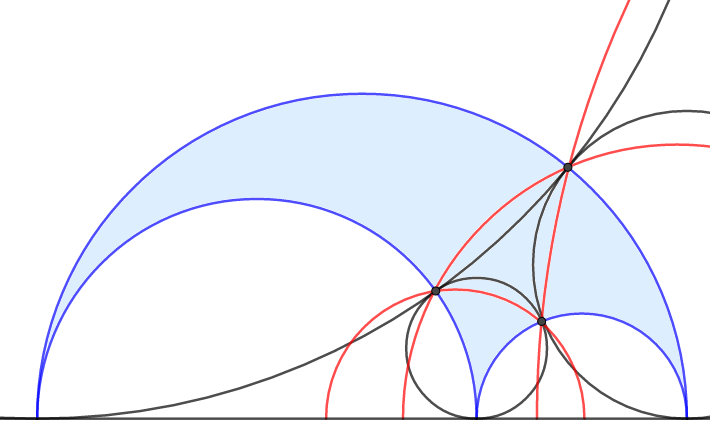
\includegraphics[width=0.5\linewidth]{pic1}
	\end{figure}
	
	